\documentclass{ltjsarticle}
\usepackage[ipaex]{luatexja-preset}
\usepackage{luatexja-fontspec}
\usepackage{color}
\usepackage{xcolor}
\definecolor{lightgray}{rgb}{0.8,0.8,0.8}
%\documentclass[]{article}
\usepackage{lmodern}
\usepackage{amssymb,amsmath}
\usepackage{ifxetex,ifluatex}
\usepackage{fixltx2e} % provides \textsubscript
\ifnum 0\ifxetex 1\fi\ifluatex 1\fi=0 % if pdftex
  \usepackage[T1]{fontenc}
  \usepackage[utf8]{inputenc}
\else % if luatex or xelatex
  \usepackage{unicode-math}
  \setmathfont{XITSMath}
  \defaultfontfeatures{Ligatures=TeX,Scale=MatchLowercase}
    \setmonofont[Mapping=tex-ansi]{Consolas}
\fi
% use upquote if available, for straight quotes in verbatim environments
\IfFileExists{upquote.sty}{\usepackage{upquote}}{}
% use microtype if available
\IfFileExists{microtype.sty}{%
\usepackage[]{microtype}
\UseMicrotypeSet[protrusion]{basicmath} % disable protrusion for tt fonts
}{}
\PassOptionsToPackage{hyphens}{url} % url is loaded by hyperref
\usepackage[unicode=true]{hyperref}
\hypersetup{
  pdftitle={テストレポート},
  pdfauthor={Sakaki},
  pdfborder={0 0 0},
  breaklinks=true}
\urlstyle{same}  % don't use monospace font for urls
\usepackage{listings}
\usepackage{courier}
\lstset{
  basicstyle=\ttfamily,
  backgroundcolor=\color{black!10},
  xleftmargin=1.0cm,
  xrightmargin=1.0cm,
  framexleftmargin=3em,
  numbers=left,
  numbersep=8pt,
  extendedchars=true,
  frame=single,
  numberstyle=\tiny,
  rulecolor=\color{black},
  numberstyle=\color{gray},
  breaklines=true,
  breakatwhitespace=true,
  breakautoindent=true,
  linewidth=\textwidth,
  keywordstyle=\color[rgb]{0,0,1},
  commentstyle=\color[rgb]{0.133,0.545,0.133},
  stringstyle=\color[rgb]{0.627,0.126,0.941},
}
\usepackage{longtable,booktabs}
% Fix footnotes in tables (requires footnote package)
\IfFileExists{footnote.sty}{\usepackage{footnote}\makesavenoteenv{long table}}{}
\usepackage{graphicx,grffile}
\makeatletter
\def\maxwidth{\ifdim\Gin@nat@width>\linewidth\linewidth\else\Gin@nat@width\fi}
\def\maxheight{\ifdim\Gin@nat@height>\textheight\textheight\else\Gin@nat@height\fi}
\makeatother
% Scale images if necessary, so that they will not overflow the page
% margins by default, and it is still possible to overwrite the defaults
% using explicit options in \includegraphics[width, height, ...]{}
\setkeys{Gin}{width=\maxwidth,height=\maxheight,keepaspectratio}
\IfFileExists{parskip.sty}{%
\usepackage{parskip}
}{% else
\setlength{\parindent}{0pt}
\setlength{\parskip}{6pt plus 2pt minus 1pt}
}
\setlength{\emergencystretch}{3em}  % prevent overfull lines
\providecommand{\tightlist}{%
  \setlength{\itemsep}{0pt}\setlength{\parskip}{0pt}}
\setcounter{secnumdepth}{0}
% Redefines (sub)paragraphs to behave more like sections
\ifx\paragraph\undefined\else
\let\oldparagraph\paragraph
\renewcommand{\paragraph}[1]{\oldparagraph{#1}\mbox{}}
\fi
\ifx\subparagraph\undefined\else
\let\oldsubparagraph\subparagraph
\renewcommand{\subparagraph}[1]{\oldsubparagraph{#1}\mbox{}}
\fi

% set default figure placement to htbp
\makeatletter
\def\fps@figure{htbp}
\makeatother


\title{テストレポート}
\author{Sakaki}
\date{2018/11/13}

\begin{document}
\maketitle
\newpage

\hypertarget{ux30d7ux30edux30b0ux30e9ux30e0}{%
\section{1. プログラム}\label{ux30d7ux30edux30b0ux30e9ux30e0}}

プログラムはこんな感じになります。

\begin{lstlisting}[language=Python]
class Device:
    type_id = TypeId.LookupByName("ns3::PacketSocketFactory")

    def __init__(self, address):
        self.address_send = self.address_receive = address
        self.socket_send = self.socket_receive = None
    
    def prepare(self, node, callback):
        self.socket_send = PacketSocket.CreateSocket(node, self.type_id)
        self.socket_send.Bind(self.address_send)
        self.socket_send.Connect(self.address_send)

        self.socket_receive = PacketSocket.CreateSocket(node, self.type_id)
        self.socket_receive.Bind(self.address_receive)
        self.socket_receive.Connect(self.address_receive)
        self.socket_receive.SetRecvCallback(callback)
    
    def send_packet(self, packet):
        return self.socket_send.Send(packet, 0)
\end{lstlisting}

\hypertarget{ux6570ux5f0f}{%
\section{2. 数式}\label{ux6570ux5f0f}}

数式はこんな感じになります。

\[\mathrm{TimesIn}(x) = \frac{\Sigma_{i=1}^{c-(x-1)}N_{i}}{T_{tw}N_x},\, \mathrm{CacheWeight}(x) = \frac{x}{c}\hspace{2cm}(1)\]

\[\mathrm{ProbCache}(x) = \mathrm{TimesIn}(x) \times \mathrm{CacheWeight}(x)\hspace{2cm}(2)\]

\hypertarget{ux56f3ux8868}{%
\section{3. 図表}\label{ux56f3ux8868}}

表はこんな感じになります。

\begin{longtable}[]{@{}ccccc@{}}
\caption{テスト}\tabularnewline
\toprule
スペクトル線 & 次数 &  \(\theta_m\)  & \(N / \,\mathrm{mm^{-1}}\) &
\(\Delta N / \,\mathrm{mm^{-1}}\)\tabularnewline
\midrule
\endfirsthead
\toprule
スペクトル線 & 次数 &  \(\theta_m\)  & \(N / \,\mathrm{mm^{-1}}\) &
\(\Delta N / \,\mathrm{mm^{-1}}\)\tabularnewline
\midrule
\endhead
\(D_1\) & 1 & \(20^{\circ}\,43'\,05''\) & \(599.99\) &
\(0.46\)\tabularnewline
\(D_1\) & 2 & \(45^{\circ}\,05'\) & \(599.92\) & \(0.17\)\tabularnewline
\(D_2\) & 1 & \(20^{\circ}\,56'\) & \(600.36\) & \(0.46\)\tabularnewline
\(D_2\) & 2 & \(45^{\circ}\,00'\) & \(600.53\) & \(0.17\)\tabularnewline
\bottomrule
\end{longtable}

図はいろいろとずれるので最後にまとめて置いた方が良いです。

また、図表番号は順番に付いていくようですが、文中で動的に参照する方法があるかはちょっと分かりません。R
markdownだと\href{https://rmarkdown.rstudio.com/authoring_basics.html}{このサイト}に書いてある感じでいけるらしいですが・・・

\begin{figure}
\centering
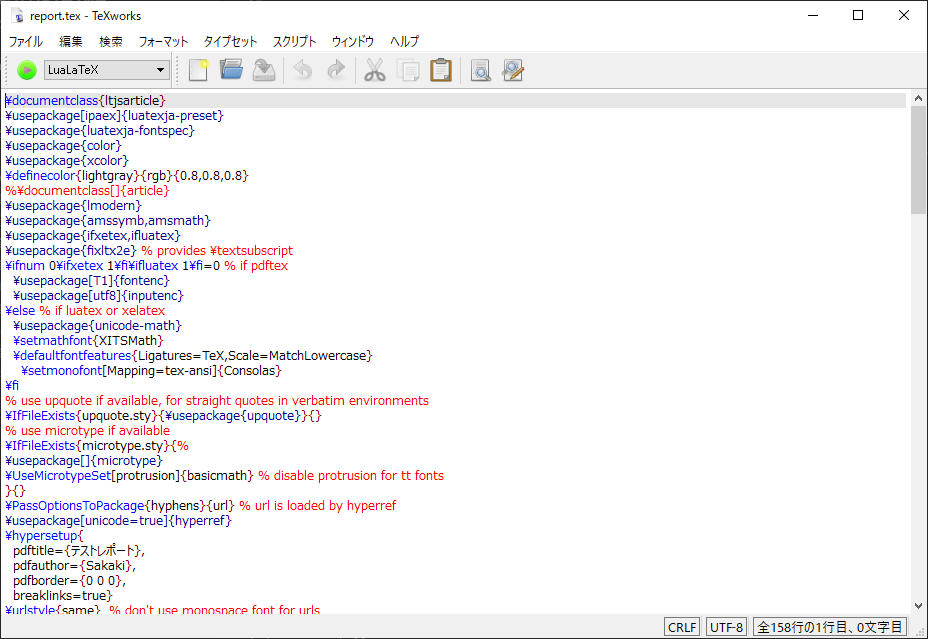
\includegraphics[width=10cm,height=\textheight]{fig1.png}
\caption{テストの図}
\end{figure}

\end{document}
